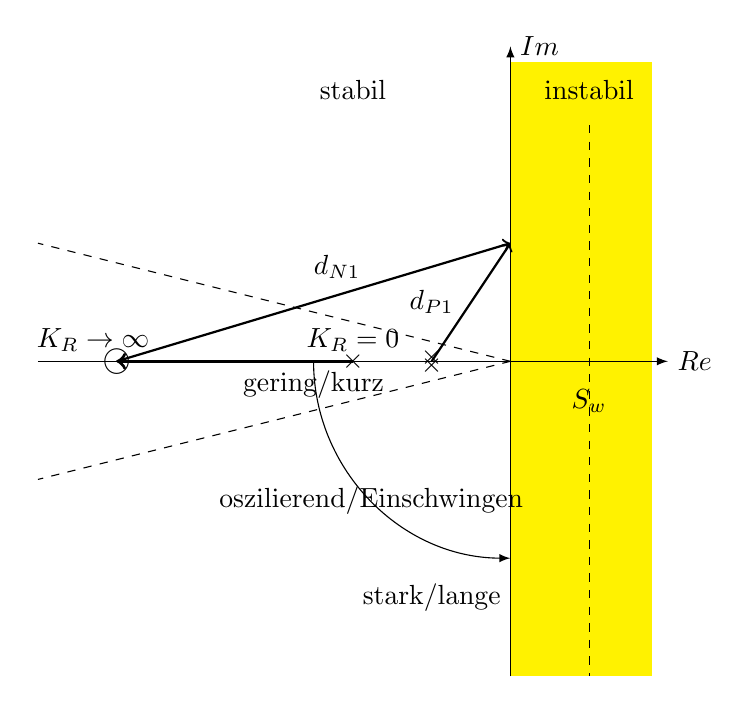
\begin{tikzpicture}
    \fill [yellow] (0,3.8) rectangle (1.8,-4);
    \draw[-latex](0,-4)--(0,4) node[right]{$Im$};
    \draw[-latex](-6,0)--(2,0) node[right]{$Re$};
    \node[above] at (-2,3.2) {stabil};
    \node[above] at (1,3.2) {instabil};
    
    \draw[dashed](0,0)--(-6,1.5);
    \draw[dashed](0,0)--(-6,-1.5);

    \draw[-latex] (-2.5,0) arc(180:270:2.5) node[midway]{oszilierend/Einschwingen}; 
    \node[below] at (-2.5,0) {gering/kurz};
    \node[left] at (0,-3) {stark/lange};

    \draw[->,very thick](-2,0)--(-5,0) node[]{$\bigcirc$};
    \node[] at (-2,0) {$\times$};
    \node[above] at (-2,0) {$K_R = 0$};
    \node[above] at (-5.3,0) {$K_R \rightarrow \infty$};

    \draw[dashed](1,3)--(1,-4) node[midway]{$S_w$};
    \node[] at (-1,0.05) {$\times$};
    \node[] at (-1,-0.05) {$\times$};
    \draw[->,thick](-1,0)--(0,1.5) node[midway, xshift=-0.5cm]{$d_{P1}$};
    \draw[->,thick](-5,0)--(0,1.5);
    \node[] at (-2.2,1.2) {$d_{N1}$};
\end{tikzpicture}